% Write the full path to the location of the graphics relative to book.tex
\graphicspath{{chapters/chp1/graphics/}}

\linenumbers

\title{The FEniCS Project on AWS Graviton3}
\titlerunning{The FEniCS Project on AWS Graviton3}

\author{M.~Habera and J.~S.~Hale}
\authorrunning{Habera and Hale}

\institute{M.~Habera \email{michal.habera@rafinex.com} \at Rafinex SARL, Luxembourg and Institute of Computational Engineering, Department of Engineering, Faculty of Science, Technology and Medicine, University of Luxembourg, Luxembourg.\\
J.~S.~Hale \email{jack.hale@uni.lu} \at Institute of Computational Engineering, Department of Engineering, Faculty of Science, Technology and Medicine, University of Luxembourg, Luxembourg.}

\maketitle

\abstract{ARM architecture central processing units are increasingly prevalent
in high performance computers due to their energy efficiency, scalability and
cost-effectiveness. The overall goal of this study is to evaluate the
suitability of ARM-based cloud computing instances for executing finite element
computations. Specifically, we show performance results executing the FEniCS
Project finite element software on Amazon Web Services (AWS) c7g and c7gn
instances with Graviton3 processors. These processors support ARMv8.4-A
instruction set with Scalable Vector Extensions (SVE) for Single Instruction
Multiple Data operations and the Elastic Fabric Adaptor for communications
between instances. Both clang 18 and GCC 13 compilers successfully generated
optimized code using SVE instructions which ensures that users can achieve
optimized performance without extensive manual tuning. Testing a distributed
memory parallel DOLFINx Poisson solver with up to 512 Message Passing Interface
processes, we found that the performance and scalability of the AWS instances
are comparable to a dedicated AMD EPYC Rome cluster installed at the University
of Luxembourg. These findings demonstrate that ARM-based cloud computing
instances, exemplified by AWS Graviton3, can be competitive for distributed
memory parallel finite element analysis.}

\section*{Introduction}

The FEniCS Project~\citep{alnaes2015fenics,baratta_dolfinx_2023} has been used
to write finite element solvers for problems arising in fields that involve the
solution of partial differential equations (PDEs), including mathematics,
biology, physics, engineering, geophysics and mechanics.

Exploring ARM-based processors and cloud computing instances for executing
FEniCS Project-based solvers is worthwhile due to ARMs potential advantages in
cost-effectiveness, energy efficiency and scalability with respect to
x86-64-based machines~\cite{simakov_are_2023,suarez_comprehensive_2024}.
Examples of adoption of ARM in the HPC space include the Isambard project
(Isambard 3, NVIDIA Grace, \citep{isambard}), Mont-Blanc project (Phase 3,
Cavium Thunder X2, \citep{Rajovic2016}), Fugaku supercomputer (Fujitsu A64FX,
\citep{fugaku}) and Astra supercomputer (Cavium Thunder X2, \citep{astra}). The
publically available cloud services with ARM instances include Amazon Web
Services (AWS) (Graviton3 CPU based on Neoverse V1 and Graviton4 CPU with
Neoverse V2), Google Cloud (Axion CPU based on Neoverse V2,
\citep{google_arm_compute}) and Microsoft Azure (Azure Cobalt 100 based on
Neoverse N2, \citep{microsoft_azure}).

AWS Graviton3-based instances aim to provide cost effective compute resources
for scientific computing and machine-learning applications by including both
Scalable Vector Extension (SVE) instructions for Single Instruction Multiple
Data (SIMD) parallelism and the Elastic Fabric Adaptor (EFA) interconnect for
high-bandwidth low-latency communication between instances. This makes the AWS
cloud offering particularly appealing for executing scientific computing codes,
like the FEniCS Project.

A key technology in the FEniCS Project is the use of automatic code generation
(compilation). The user expresses their finite element problem in the Unified
Form Language (UFL)~\citep{alnaes_unified_2014} and then the FEniCSx Form
Compiler (FFCx)~\citep{kirby_compiler_2006} compiles the UFL description of the
problem into a low-level C kernel for computing the cell-local finite element
tensor.

One aspect of good performance of a compute-bound kernel is ensuring the
assembly code of the compiled kernel contains calls to Single Instruction
Multiple Data (SIMD) operations. SIMD operations can apply the same operation
to multiple data items in a single CPU clock cycle. For a recent overview of
SIMD programming strategies see e.g. \citep{rocke_evaluation_2023}. The current
strategy of FFCx with respect to SIMD is to ensure that its kernels are
amenable to the compiler applying automatic vectorisation, a process that
automatically converts a scalar program into a vectorised equivalent that uses
SIMD operations.
 
Consequently for users to achieve good performance when using FEniCSx on
Graviton3 it is important to verify that the latest compilers do automatically
emit SVE and/or Neon SIMD instructions when compiling the generated C finite
element kernels and that these kernels achieve reasonable runtime performance. 

In addition to SIMD parallelisation at the kernel level, DOLFINx, the finite
element problem solving environment of the FEniCS Project, also supports
distributed memory parallel assembly of global finite element data structures
(sparse matrices and vectors) using the Message Passing Interface (MPI), for
full details see \cite{baratta_dolfinx_2023}. For user's to run large-scale
DOLFINx simulations on AWS it is necessary to verify that the EFA interconnect
provides sufficient performance for parallel scalability.

In summary, the contribution of this chapter is to examine both SIMD
performance and multi-node parallel scaling of the FEniCS Project software on
Amazon's Graviton3 based instances. 

\section*{Methodology and Results}

\subsection*{Systems}
AWS c7g and c7gn instances are compared to Aion computing instances available
at the University of Luxembourg HPC facilities \citep{VCPKVO_HPCCT22}. These
instances have different hardware configuration, see
\autoref{tab:aion-aws-config} for full details.

The FEniCS Project components are written in a mixture of Python, modern-style
C++20 and Standard C17. The Python interface is a wrapper around the core data
structures and computationally intensive algorithms written in C and C++.

\begin{table}
  \footnotesize
  \renewcommand{\arraystretch}{1.5}
  \begin{tabular}{l|l|l}
                              & Aion node                                                          & AWS c7g instance \\ \hline \hline
    Processor                 & \makecell[l]{2 x (AMD Epyc ROME 7H12, \\ 64 cores @ 2.6 GHz)}      & \makecell[l]{1 x (Graviton3, \\ 64 cores @ 2.6 GHz)} \\ \hline
    Architecture              & x86\_64, Zen 2 (AVX2)                                              & ARMv8.4-A, Neoverse V1 (SVE) \\ \hline
    Memory                    & \makecell[l]{256 GB DDR4 \\ 3200 MT/s = 25.6 GB/s \\ 8 NUMA nodes} & \makecell[l]{128 GB DDR5 \\ 4800 MT/s = 38.4 GB/s  \\ Unified Memory Access (no NUMA) } \\ \hline
    Total mem. bandwidth      & 2 x 200 GB/s                                                       & 1 x 300 GB/s  \\ \hline
  \end{tabular}
  \vspace{5pt}
  \caption{Configuration of the Aion nodes (University of Luxembourg HPC) and
	AWS c7g (Amazon) instances. The c7gn instance used in the Poisson weak
	scaling test has the same hardware as c7g with the addition of a
	$\SI{200}{\giga\byte\per\second}$ interconnect between instances for
	MPI-based communication.}
  \label{tab:aion-aws-config}
\end{table}

\subsection*{Memory bandwidth}

Low-order finite element methods are typically memory bandwidth constrained as
the time taken to load and store data from main memory (e.g. the mesh geometry)
dominates the time taken to perform the arithmetic operations to compute the
finite element cell tensor. Understanding the memory bandwidth characteristics
of a processor is therefore important for ensuring optimal performance.

STREAM \citep{McCalpin1995,McCalpin2007} is the industry standard benchmark for
measuring sustained memory bandwidth performance. They estimate memory bandwidth
from memory intense operations (copy, scale, add) on large contiguous arrays.

In \autoref{fig:stream-single} results for the copy operation for single-node
benchmark are shown. For the single-node benchmark $\SI{80}{\percent}$ of the
theoretical peak memory bandwidth of $\SI{400}{\giga\byte\per\second}$ for Aion
and $\SI{300}{\giga\byte\per\second}$ for AWS c7g is reached. This is considered
a reasonable outcome of the STREAM benchmark, \citep{McCalpin2023}. Bandwidth
saturation is observed at around $\SI{20}{\percent}$ of the node utilisation.
Both curves show different characteristics of the saturation point due to
different memory access configuration. On the Aion instances there are 8
non-unified memory access (NUMA) nodes of 16 cores each, while AWS c7g instances
are setup with unified memory access.

\begin{figure}
\begin{center}
        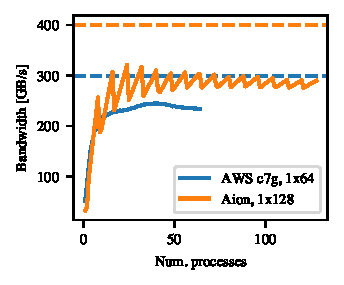
\includegraphics{chapters/chp1/graphics/stream_plots/stream_single_node.pdf}
\end{center}
	\caption{Single-node STREAM benchmark. Theoretical peak bandwidth of each system show as dashed line.}
        \label{fig:stream-single}
\end{figure}

\subsection*{Finite element kernels}

In order to measure the performance of a standard FEniCS user finite element
code we used the Local Finite Element Operator Benchmarks repository
\citep{Baratta2023}. The benchmark measures execution time for local finite
element kernel generated by the FEniCS Form Compiler (FFCx) v0.9.0
\citep{kirby_compiler_2006}. We generate a matrix-free three-dimensional
Laplace kernel representing a finite element discretisation of the action of
Laplace operator $A_{ij}$ with spatially varying material property $\kappa(x)$
\begin{align}
    v_i = A_{ij} w_j, \quad
    A_{ij} = \int_K \kappa J_{mk} J_{mn} \nabla_k \phi_i \nabla_n \phi_j |\det J| \mathrm dx,
\end{align}
where $K$ is a fixed reference tetrahedron, $w_j \in \mathbb{R}^{n}$ is a
fixed, prescribed vector, $J$ is a Jacobian transformation matrix and $\phi$
are finite element basis functions.

The generated kernel calculates a double precision vector $v_i \in
\mathbb{R}^{n}$, where $n = 4$ for first-order discretization (low-order) and
$n = 165$ for eight-order discretization (high-order). Low-order kernels are
expected to be memory bandwidth limited, while high-order kernels have higher
arithmetic intensity. In addition, the matrix-free (operator action) version
requires fewer load and store operations in comparison to the assembly of a
matrix, increasing the ratio of floating-point operations to memory loads and
stores. Consequently for the high-order kernels there is the scope for
significant performance increases if the compiler can automatically emit SIMD
operations.

\subsubsection*{Generated code structure}

Compiler (loop) SIMD auto-vectorisation is usually performed for inner-most
loops with compile-time known bounds. The analysis of FFCx autogenerated code
is required to understand the potential and missed optimisations.

\lstset{style=CStyle}
\begin{lstlisting}[language=c,
    caption=Abbreviated FFCx generated finite element kernel.,
    basicstyle=\ttfamily\scriptsize,
    keywordstyle=\ttb\color{deepblue}\scriptsize,
    label=lst:c-code]
void kernel(double* restrict A, const double* restrict w, ...){
    // 1. Static arrays of basis functions and quadrature weights.
    // 2. Quadrature rule independent computations.

    for (int iq = 0; iq < NUM_QUAD_POINTS; ++iq) {
        // 3. Quadrature loop body.
        for (int ic = 0; ic < NUM_DOFS; ++ic){
            // 3.1 Coefficient evaluation.
            w1_d100 += w[4 + (ic)] * FE0_C0_D100_Q530[0][0][iq][ic];
            // ...
        }

        // 3.2 Scalar graph evaluation.
        double sv_530_0 = w1_d100 * sp_530_18;
        double sv_530_1 = w1_d010 * sp_530_22;
        // ...

        for (int i = 0; i < NUM_DOFS; ++i) {
            // 3.3 Tensor assignment loop.
            A[(i)] += fw0 * FE0_C0_D100_Q530[0][0][iq][i];
            // ...
        }
    }
}
\end{lstlisting}

An abbreviated example of generated C code is shown in Code Listing
\ref{lst:c-code}. Firstly, there are arrays defining finite element basis
functions at quadrature points. These require no arithmetic operations.
Computations independent of the quadrature loop contain more intense arithmetic
operations (e.g. determinant of the Jacobian), but are executed only once.
Non-affine geometry would require evaluation of geometric quantities at each
quadrature point, which would increase the arithmetic intensity and yield more
opportunities for vectorisation.

The most performance critical part of the code is contained in the quadrature
loop body. For the eight-order Laplace operator there is
\lstinline{NUM_QUAD_POINTS = 214} and \lstinline{NUM_DOFS = 165}. There are two
inner-most loops: coefficient evaluation and tensor assignment. Both contain a
set of multiply-add operations which are candidates for automatic vectorisation
via fused multiply-add operations in both SVE (Graviton3) and AVX2 (AMD EPYC).

\subsubsection*{Experimental results}

For the finite element kernel benchmarks we compiled the kernels with
LLVM/clang 18.1.3 and GCC 13.2.0. Full details are given in
\autoref{tab:compilers-kernels}.

\begin{table}
    \centering
    \footnotesize
    \renewcommand{\arraystretch}{1.5}
    \begin{tabular}{l|l|l|l}
                                    & Compiler     & Aion                                                                                            & AWS c7g \\ \hline \hline
        Ofast, native, vectorized   & GCC 13.2.0   & \makecell[l]{-Ofast \\ -march=znver2 \\ -mtune=znver2}                                          & \makecell[l]{-Ofast \\ -mcpu=neoverse-v1} \\ \hline
                                    & clang 18.1.3 & \makecell[l]{-Ofast \\ -march=znver2 \\ -mtune=znver2}                                          & \makecell[l]{-Ofast \\ -mcpu=neoverse-v1} \\ \hline
        Ofast, native, no vec.      & GCC 13.2.0   & \makecell[l]{-Ofast \\ -march=znver2 \\ -mtune=znver2 \\ -fno-tree-vectorize}                   & \makecell[l]{-Ofast \\ -mcpu=neoverse-v1 \\ -fno-tree-vectorize} \\ \hline
                                    & clang 18.1.3 & \makecell[l]{-Ofast \\ -march=znver2 \\ -mtune=znver2 \\ -fno-slp-vectorize \\ -fno-vectorize}  & \makecell[l]{-Ofast \\ -mcpu=neoverse-v1 \\ -fno-slp-vectorize \\ -fno-vectorize} \\ \hline
        O2, no vec.                 & GCC 13.2.0   & \makecell[l]{-O2 \\ -fno-tree-vectorize}                                                        & \makecell[l]{-O2 \\ -fno-tree-vectorize} \\ \hline
                                    & clang 18.1.3 & \makecell[l]{-O2 \\ -fno-slp-vectorize \\ -fno-vectorize}                                       & \makecell[l]{-O2 \\ -fno-slp-vectorize \\ -fno-vectorize} \\ \hline
    \end{tabular}
    \vspace{5pt}
    \caption{Compiler versions and compilation flags used for finite element kernel benchmarks.}
    \label{tab:compilers-kernels}
\end{table}

Results for kernel benchmarks are shown in \autoref{fig:local-deg1}
and \autoref{fig:local-deg8}. Low-order kernels (\autoref{fig:local-deg1}) show no
dependence on compiler vectorisation setup. On the other hand, AWS c7g shows
1.3x speed-up over Aion which we attribute to higher memory bandwidth for a
single process.

High-order kernels (\autoref{fig:local-deg8}), which are expected to benefit from
SIMD operations, show a clear link between compiler settings and performance.
Both clang and GCC auto-vectorisers perform well, producing a noticeable
speed-up (\textgreater 2x) in the most optimised setting. The vectorisation
speed-up (\textgreater 4x) is more significant with the Aion nodes.

\begin{figure}
    \begin{subfigure}{.5\textwidth}
        \centering
        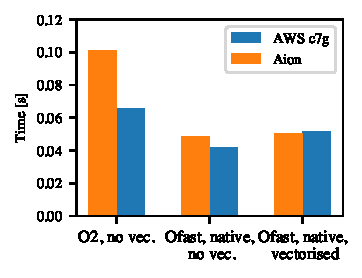
\includegraphics{chapters/chp1/graphics/kernel_plots/local_operator_clang_deg1.pdf}
        \caption{clang 18.1.3.}
        \label{fig:local-clang-deg1}
    \end{subfigure}%
    \begin{subfigure}{.5\textwidth}
        \centering
        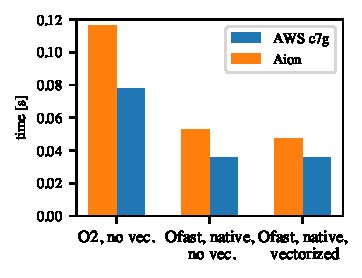
\includegraphics{chapters/chp1/graphics/kernel_plots/local_operator_gcc_deg1.pdf}
        \caption{GCC 13.2.0.}
        \label{fig:local-gcc-deg1}
    \end{subfigure}
    \caption{Low-order Laplace operator action assembly.}
    \label{fig:local-deg1}
\end{figure}

\begin{figure}
    \begin{subfigure}{.5\textwidth}
        \centering
        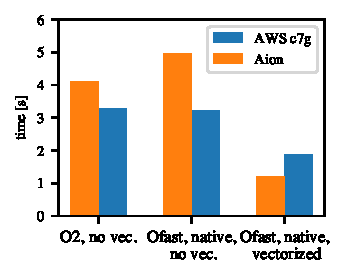
\includegraphics{chapters/chp1/graphics/kernel_plots/local_operator_clang_deg8.pdf}
        \caption{clang 18.1.3.}
        \label{fig:local-clang-deg8}
    \end{subfigure}%
    \begin{subfigure}{.5\textwidth}
        \centering
        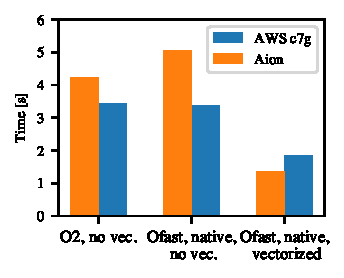
\includegraphics{chapters/chp1/graphics/kernel_plots/local_operator_gcc_deg8.pdf}
        \caption{GCC 13.2.0.}
        \label{fig:local-gcc-deg8}
    \end{subfigure}
    \caption{High-order Laplace operator action assembly.}
    \label{fig:local-deg8}
\end{figure}

Optimisation reports (\texttt{-Rpass=loop-vectorize} for clang,
\texttt{-fopt-info-vec-optimized} for GCC) and the inspection of the generated
assembly reveal that the low-order operator action the compiler optimisation
level \lstinline{-Ofast} makes constant folding more effective and pre-computes
more operations at compile-time (e.g. partial sums of the static constant arrays)
\citep{GodboltArmClangDeg1}.

On Graviton3, both GCC and clang generate SVE FMLA instructions
\citep{ArmReferenceManual} for both the coefficient evaluation and tensor
assignment loops \citep{GodboltArmClang,GodboltArmGCC}. FMLA, or Floating-point
fused Multiply-Add, is a SIMD instruction that multiplies two vectors stored in
SVE registers and adds the result to a third vector. The coefficient evaluation
loop with no interdependencies between iterations is a perfect example for
compiler auto-vectorisation. Moreover, for coefficients of higher order
discretization, there is potential for exploiting wider SVE registers (up to
2048 bits).

An assembly excerpt for the coefficient evaluation is shown below.
\begin{lstlisting}[
    basicstyle=\ttfamily\footnotesize,
    keywordstyle=\ttb\color{deepblue}\footnotesize]
ld1d    {z0.d}, p0/z, [x7, x0, lsl #3]
ld1d    {z25.d}, p0/z, [x3, x0, lsl #3]
fmla    z3.d, p0/m, z25.d, z0.d
...
faddv   d1, p1, z1.d
\end{lstlisting}
As expected, there are two contiguous loads LD1D into two of the available SVE
Z0-Z31 registers followed by a fused Multiply-Add instruction. The result is
accumulated into an SVE register Z3 which is then horizontally summed outside
of the vectorised loop (FADDV). Here P0 is a predicate register without any
constraints on the available elements.

On Aion, both GCC and clang vectorise both coefficient evaluation and tensor
assignment loops and rely on the \lstinline{VFMADD231PD} instructions on the
YMM registers, i.e. vectorisation width of 4 doubles
\citep{Godboltx86Clang,Godboltx86GCC}.

\subsection*{Parallel scalability}

Results for the parallel scalability were produced using performance test codes
for FEniCSx \citep{Wells2023} built against DOLFINx 0.6.0 and PETSc 3.18
\citep{petsc} with the Spack package manager setup to use GCC 12.2.0. We setup
Spack to use a version of OpenMPI provided by AWS which includes the appropriate
libfabric with native support for the EFA interconnect. Libfabric is a network
communication library that abstracts networking technologies from fabric and
hardware implementation, ensuring optimal data transfer across Amazon's
proprietary EFA interconnect.

The Poisson equation solver benchmark consists of the following measured steps:
\begin{enumerate}
    \item Create mesh. Create a unit cube mesh and discretise using linear
    tetrahedral cells. Partition the mesh with Parmetis 4.0.3 partitioner
    \citep{Karypis1998} and distribute.
    \item Assemble matrix. Execute the local Poisson equation kernel over the
    mesh and assemble into a PETSc MATMPIAIJ (distributed compressed sparse row)
    matrix.
    \item Solve. Run Conjugate Gradient (CG) solver with a classical algebraic
    multigrid (BoomerAMG \citep{hypre}) preconditioner.
\end{enumerate}
%
Weak scaling results (constant workload of approx. \SI{5e+5} degrees-of-freedom
per process) are shown in \autoref{fig:weak-scaling}. Both Aion and AWS c7gn
show almost constant times for mesh creation ($< 5\%$ difference).

Matrix assembly is expected to have ideal weak parallel scalability due to the
cell-local nature of the assembly loop and negligible amount of MPI
communication during matrix finalisation. Aion and AWS c7gn show small increase
in time (10-15 \%) for 512 processes.

The time for the solve step increases by 40 \% for 512 processes on AWS c7gn and
by 27 \% on Aion. However, the number of Krylov iterations of the preconditioned
CG solver grows from 16 to 20 for 512 processes (25\% increase) due to the
inefficiency of the algebraic multigrid preconditioner on an unstructured 3D
mesh. Taking this into account, the time per iteration is almost constant on
Aion ($< 5\%$) and a small increase of 15 \% on AWS c7gn is observed.

\begin{figure}
    \begin{subfigure}{.7\textwidth}
	\begin{center}
        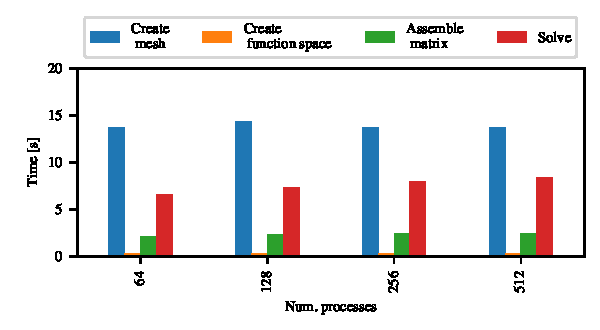
\includegraphics{chapters/chp1/graphics/parallel_scaling_plots/output/weak_scaling_aion_poisson.pdf}
        \caption{Aion, \SI{5e+5} degrees-of-freedom per process, 25 \% utilisation (32 processes per node).}
        \label{fig:weak-scaling-aion}
	\end{center}
    \end{subfigure}

    \begin{subfigure}{.7\textwidth}
	\begin{center}
        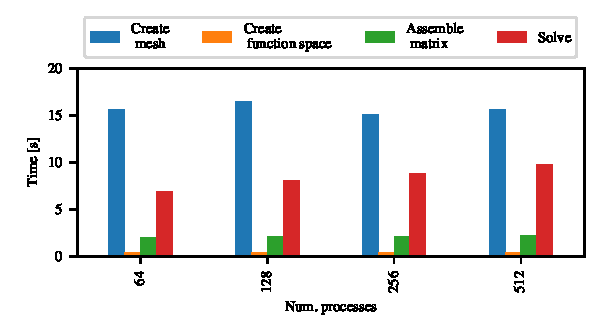
\includegraphics{chapters/chp1/graphics/parallel_scaling_plots/output/weak_scaling_aws_c7gn_poisson.pdf}
        \caption{AWS c7gn, \SI{5e+5} degrees-of-freedom per process, 50 \% utilisation (32 processes per node).}
        \label{fig:weak-scaling-aws}
	\end{center}
    \end{subfigure}
    \caption{Weak parallel scalability of the DOLFINx Poisson equation solver on Aion and AWS c7gn systems.}
    \label{fig:weak-scaling}
\end{figure}

\section*{Conclusions}

Benchmarks for memory bandwidth, local finite element kernels and parallel
scalability of Poisson solver were executed on Aion nodes and on AWS c7g(n)
instances.

Memory bandwidth measured using STREAM MPI confirms higher memory transfer rate
of AWS c7g(n), but a superior total bandwidth of
~\SI{310}{\giga\byte\per\second} per Aion node.

In terms of auto-vectorisation capabilities of GCC 13.2.0 and clang 18.1.3, both
produced optimised instructions for the targeted microarchitectures (Zen 2 for
Aion and Neoverse V1 for AWS c7g). This observation was confirmed with
performance benchmarks based on local finite element kernels for the Laplace
operator.

The MPI-based distributed memory Poisson equation solver shows weak scaling with
15 \% time per iteration increase for 512 processes on the c7gn-based cluster.
Results for the in-house University of Luxembourg Aion system are slightly
superior with almost constant ($< 5 \%$) time per iteration for 512 processes.

Based on our results, we conclude that AWS Graviton3 instances are a viable
alternative for high-performance computing tasks using the FEniCS Project
automated finite element solver. These instances are likely to be particularly
interesting for users with infrequent or highly elastic large-scale
computational demands~\cite{emeras_amazon_2016}.

In future work we plan to work on other more complex problems (e.g. linear
elasticity) and performance benchmarks of direct solvers. Additionally, the
latest generation Graviton4 instances provide an improved Neoverse V2
instruction set, which has a smaller SVE vector length of 128 bits,
\citep{ArmReferenceManualNeoverseV2}, which warrants further investigation.

\section*{Supplementary material}
Raw data and plotting scripts are archived at \citep{habera_2024_13748405}.

\begin{acknowledgement}
This project has received compute resources from Amazon Web Services (AWS)
through the first and second collaborative University of Luxembourg and
AWS Graviton3 call. The experiments presented in this paper were
carried out using the HPC facilities of the University of Luxembourg
~\cite{VCPKVO_HPCCT22} {\small -- see \url{https://hpc.uni.lu}}

This research was funded in whole, or in part, by the National Research
Fund (FNR), grant reference COAT/17205623. For the purpose of open
access, and in fulfillment of the obligations arising from the grant
agreement, the author has applied a Creative Commons Attribution 4.0
International (CC BY 4.0) license to any Author Accepted Manuscript
version arising from this submission.
\end{acknowledgement}

\bibliographystyle{spbasic}
\bibliography{chapters/chp1/bibliography.bib}
